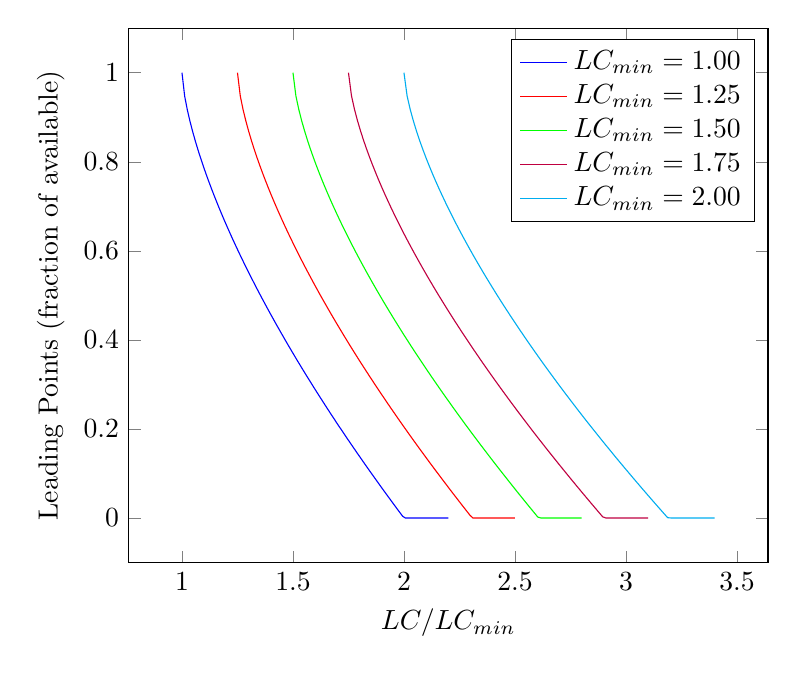
\begin{tikzpicture}
\begin{axis}[ xlabel=$LC/LC_{min}$
            , ylabel=Leading Points (fraction of available)
            , width=0.8\textwidth
            , xtick={ 1, 1.5, 2, 2.5, 3, 3.5 }
            ]
    \addplot[ blue
            , domain=1:2.2
            , samples=100
            ]{max(0, 1 - ((x - 1)^2/1^(1/2))^(1/3))};
    \addplot[ red
            , domain=1.25:2.5
            , samples=100
            ]{max(0, 1 - ((x - 1.25)^2/1.25^(1/2))^(1/3))};
    \addplot[ green
            , domain=1.5:2.8
            , samples=100
            ]{max(0, 1 - ((x - 1.5)^2/1.5^(1/2))^(1/3))};
    \addplot[ purple
            , domain=1.75:3.1
            , samples=100
            ]{max(0, 1 - ((x - 1.75)^2/1.75^(1/2))^(1/3))};
    \addplot[ cyan
            , domain=2:3.4
            , samples=100
            ]{max(0, 1 - ((x - 2)^2/2^(1/2))^(1/3))};
    \legend{ $LC_{min} = 1.00$
           , $LC_{min} = 1.25$
           , $LC_{min} = 1.50$
           , $LC_{min} = 1.75$
           , $LC_{min} = 2.00$
           }
\end{axis}
\end{tikzpicture}
